\section*{2010}
\vspace{-.5cm}
\hrulefill \smallskip\\
\ques{1}{d}{12} Solve graphically the following linear programming problem:
\begin{gather*}
    \text{Min} \enskip Z \: = \:3x_1 + 5x_2 \\
    \begin{aligned}
        \text{Subject to} \enskip 
        -3&x_1 + 4x_2 \leq 12 \\
        2&x_1 - x_2  \geq -2 \\
        &x_1 + 4x_2 \geq 12 \\
        &x_1 \leq 4,\enskip x_2\geq 2, \\
        &x_1,x_2 \geq 0.
    \end{aligned}
\end{gather*}
\myline
\ques{2}{a}{10} Explain assignment problem and transportation problem. Give its mathematical formulation.
\myline
\ques{2}{c}{10} State and prove the fundamental theorem of game theory.
\myline
\ques{3}{a}{25} For any zero-sum two-person game where the optimal strategies are not pure strategies and for which $A's$ pay-off matrix is 
\begin{figure}[h]
    \centering
    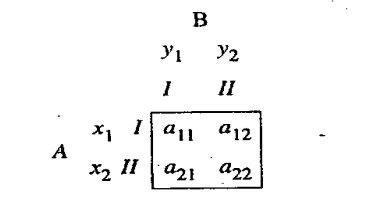
\includegraphics[]{OPT/LPTAGT/3a2010.PNG}
\end{figure} Show that the optimal strategies are $(x_1,x_2)$ and $(y_1,y_2)$ given by \[ \frac{x_1}{x_2} = \frac{a_{22}-a_{21}}{a_{11}-a_{12}} \text{ and } \frac{y_1}{y_2} = \frac{a_{22} - a_{12}}{a_{11} - a_{21}} \] and the value of the game to $A$ is given by \[v = \frac{a_{11}a_{22} - a_{12}a_{21}} {(a_{11}+a_{22}) -(a_{12}+a_{21})}.\]
\myline
\ques{4}{a}{25} A firm manufacturing a single product has three plants $X$, $Y$ and $Z$. The three plants have produced 60, 35 and 40 units respectively during this month. The firm had made commitment to sell 22 units to customer $A$, 45 units to customer $B$, 20 units to customer $C$ and 18 units to customer $D$ and 30 units to customer $E$. Determine the minimum possible transportation cost of shifting the manufactured products to five customers. The net per unit cost of transporting from the three plants to five customers is given below:
\begin{center}
    \begin{tabular}{c|*{6}{c|}}
    \multicolumn{2}{c}{} & \multicolumn{5}{c}{Customer} \\ \cline{2-7}
    & & $A$ & $B$ & $C$ & $D$ & $E$ \\ \cline{2-7}
    \multirow{3}{*}{Plant} & $X$ & 4 & 1 & 3 & 4 & 4 \\ \cline{2-7}
    & $Y$ & 2 & 3 & 2 & 2 & 3 \\ \cline{2-7}
    & $Z$ & 3 & 5 & 2 & 4 & 4 \\ \cline{2-7} 
    \end{tabular}
\end{center}